% Minimal retained preamble for lane-p2 cards taken from
% sources/hitting-sets-hypergraphs-2307.12154v3/source0.tex (arXiv:2307.12154v3).
%
% Copied verbatim from the author's own file:
%   line 3      : \documentclass[11pt,oneside]{amsart}
%   lines 43-49 : the author's macro definitions
%   lines 53-59 : the author's theorem declarations
% The base packages amsmath, amsfonts and amssymb are supplied here because amsart
% does not load amssymb by itself (LANE_BRIEF 18.1).
%
% Omitted author preamble lines and why (nothing was renamed or redefined):
%   line 10 (\usepackage[utf8]{inputenc}), line 11 (fontenc), line 12 (lmodern):
%       input encodings and font encodings fight the forced xelatex engine;
%   line 13 (geometry), line 34 (\baselinestretch), line 29 (parskip): pure layout,
%       and the assembler supplies the page setup;
%   lines 14-24 and 28 and 32 (array, fancyhdr, graphicx, float, caption, pgf, tikz,
%       tikzlings-addons, tikzlings-penguins, subcaption, adjustbox, verbatim): none of
%       the retained spans draws or floats anything, and the tikzlings package is not
%       part of the host TeX Live;
%   line 62 (\freefootnote): the retained spans contain no footnote.
\documentclass[11pt,oneside]{amsart}
\usepackage{amsmath}
\usepackage{amsfonts}
\usepackage{amssymb}

\newcommand{\R}{\mathbb{R}}
\newcommand{\N}{\mathbb{N}}
\newcommand{\HH}{\mathcal{H}}
\newcommand{\RR}{\mathcal{R}}
\newcommand{\A}{\mathcal{A}}
\newcommand{\B}{\mathcal{B}}
\newcommand{\est}{\emptyset}

\newtheorem{theorem}{Theorem}
\newtheorem{proposition}{Proposition}
\newtheorem{corollary}{Corollary}
\newtheorem{lemma}{Lemma}
\newtheorem{definition}{Definition}
\newtheorem{jel}{Notation}
\newtheorem{conj}{Conjecture}
\usepackage{graphicx}
\usepackage{verbatim}
\usepackage{cleveref}
\crefname{originaltheorem}{original theorem}{original theorems}
\Crefname{originaltheorem}{Original theorem}{Original theorems}
\makeatletter
\newlabel{vegtelen_sorozat}{{6}{source}{}{sourcepointer-1}{}}
\newlabel{vegtelen_sorozat@cref}{{[originaltheorem][0][]6}{[1][0][]source}{}{}{}}
\makeatother
\title{Bounds and infinitude for the polychromatic threshold of finite arithmetic progressions}
\author{Balázs Bursics, Bence Csonka, Luca Szepessy}
\date{arxiv:2307.12154v3; CC BY 4.0}
\begin{document}
\maketitle
\noindent\textit{Editorial note.} The counted unit is the article's own Theorem veges\_sorozat at source lines 346-359, a statement with two enumerated items, together with BOTH of its proof environments: the one headed Proof of Theorem veges\_sorozat, item (1) at source lines 925-934 and the one headed item (2) at source lines 936-960. The pairing is non-adjacent in both cases, because the article collects the introduction's proofs in a later section, and it rests on the author's own named headers; both spans are listed because the statement has two items and the article proves them separately.\par\medskip
\noindent\textit{Editorial note.} The second proof contains a lemma at source lines 938-944 with its own proof at 941-944. That lemma lies inside the retained span and is therefore NOT counted as a separate unit by this lane, in keeping with the rule that nested intervals are counted once; it is retained verbatim as part of the proof of the counted theorem.\par\medskip
\noindent\textit{Editorial note.} The second proof displays Figure ferde, whose body includes the png sikvag2.png; that file is not in the source directory but is inside the article's e-print tarball, from which it was taken, and it is carried as an asset of this task. The retained preamble therefore includes graphicx, and verbatim is kept as well.\par\medskip
\noindent\textit{Editorial note.} The second proof cites the article on Delaunay graphs of point sets with respect to axis-parallel rectangles at source line 942. That entry is supplied as a task-directory fragment holding it exactly as a bibtex run on the host had formatted it from the author's own ref.bib, since the bibtex backend cannot be used in this harness.\par\medskip
\noindent\textit{Editorial note.} The retained context at source lines 128-129 is the definition of the parameter m\_H(k) and the context at 271-280 is the author's definition of the families induced by arithmetic progressions together with the shorthand used in the statement. Nothing else is retained, so the material contains no citation other than the one fragment.\par\medskip
\noindent\textit{Editorial note.} The retained preamble's remaining lines are the author's class line at source line 3, his macro definitions at source lines 43-49 and his theorem declarations at source lines 53-59, with amsmath, amsfonts and amssymb loaded explicitly for amsart.\par\medskip
\noindent\textit{Editorial note.} The retained second proof refers once to Theorem vegtelen\_sorozat, which this lane does not count; that label is therefore declared as a non-load-bearing navigation pointer so the reference resolves. Its number is the sixth of the theorem counter in this article, counted over the theorem environments at lines 192, 214, 222, 243, 251 and 320.\par\medskip
\noindent\textit{Allowed standard prerequisites (editorial).}\begin{itemize}
\item Hypergraphs induced by arithmetic progressions. For sets D and M of natural numbers, the family A of subscript D M consists of the hypergraphs on a finite set S of natural numbers whose edges are the intersections of S with finite arithmetic progressions of difference in D and whose starting points satisfy the congruence condition M; the family with the superscript infinity uses infinite progressions instead; the author's own definition is retained at source lines 271-276.. They are the two families whose thresholds the counted theorem bounds and studies, and the shorthand m of subscript D M is exactly what its statement writes.
\item The parameter m\_H(k) and its shorthand. The parameter m\_H(k) is the smallest threshold admitting polychromatic k-colourings of every member after deleting the edges of size below the threshold, and the article writes m of subscript D M for the value on the family of arithmetic progressions; retained at source lines 128-129 and 278-280.. The counted theorem asserts an upper bound and an infinitude for two such values, so both the parameter and the shorthand must be available.
\item The family of axis-parallel rectangles as a comparison. The proof of the second item reduces to a three-dimensional family of translates of octants and compares it with the family induced by axis-parallel rectangles, whose threshold is infinite by a cited theorem recorded in the article's introduction; that entry is cited inside the counted proof and is supplied with this card as a fragment of the bibtex-formatted entry.. The comparison with the rectangle family is what goes through to give the infinitude in the second item.
\end{itemize}\medskip
\ifdefined\hypertarget\hypertarget{sourcepointer-1}{}\fi
\noindent\textit{Source reference.} Original theorem 6: sources/hitting-sets-hypergraphs-2307.12154v3/source0.tex, source lines 320--320. The retained second proof names this theorem when it recalls where the injection it reuses was built. The counted theorem and its proofs do not depend on the recalled statement itself, so the name is a navigation pointer only.\par\medskip
\begin{definition} Let $\mathcal{H}$ be a hypergraph family. Denote by $m_\mathcal{H}(k)$ the smallest positive integer $m$ such that for every $H\in\mathcal{H}$ there exists a polychromatic $k$-coloring of the hypergraph $H_{\ge m}$. If there is no such $m$, set $m_{\mathcal{H}}(k)=\infty$.
\end{definition}

\begin{definition} 
Let $D,M \subseteq \mathbb{N}$ and denote by $\mathcal{A}_{D,M}$ the family of hypergraphs $A$ such that $S:=V(A) \subseteq \mathbb{N}$ is a finite set, and 
$E(A) \subseteq \{\{a_n\}_{n=0}^{k} \cap S:\{a_n\}_{n=0}^{k} \hspace{0.2 cm}\text{is a finite arithmetic} \newline \text{progression with difference} \hspace{0.2 cm}d \in D\hspace{0.2 cm} \text{such that}\hspace{0.2 cm}\exists m\in \N: a_0-md\in M\}.$

Denote by $\mathcal{A}_{D,M}^{\infty}$ the family of hypergraphs $A$ such that $S:=V(A) \subseteq \mathbb{N}$ is a finite set and $E(A) \subseteq \{\{a_n\}_{n=0}^{\infty} \cap S:\{a_n\}_{n=0}^{\infty} \hspace{0.2 cm}\text{is an infinite arithmetic progression with difference} \hspace{0.2 cm}d \in D\hspace{0.2 cm} \text{such that}\hspace{0.2 cm}\exists m\in \N: a_0-md\in M \}.$
\end{definition}

For the sake of simplicity we use the notations
$m_{D,M}(k):=m_{\mathcal{A}_{D,M}}(k)$ and
$m_{D,M}^\infty(k):=m_{\mathcal{A}_{D,M}^{\infty}}(k)$. 

\begin{theorem}\label{veges_sorozat}
\begin{enumerate}
    \item 
    Suppose that $M$ contains at most one element of every residue class modulo $t$, then
    \[
    m_{\{t^i:i \in \mathbb{N}\}, M}(k) \leq |M|(m_{\mathcal{B}}(k) -1) + 1.
    \]
    \item 
    Let $p,q$ be positive coprime integers, then
    \[
    m_{\{p^iq^j:i,j \in \mathbb{N}\},\{0\}}(k) = \infty.
    \]
\textbf{\textbf{}}\end{enumerate}
\end{theorem}

\begin{proof} [Proof of Theorem~\ref{veges_sorozat}. (1)]
Firstly, we show that $m_{\{t^i:i \in \mathbb{N}\}, \{0\}}(k) \leq m_{\mathcal{B}}(k)$. To prove this, we construct a $\phi:\mathbb{N}\to \mathbb{R}^2$ injection such that for every fixed $i, j_0$ and $j_{\text{max}}$ the set $\phi[\{j \cdot t^i: j \in \mathbb{N}^+, j_0 \leq j \leq j_{\text{max}}\}]$ can be defined by a bottomless rectangle. Denote the arithmetic sequence $j_0 \cdot t^i, \ldots, j_{\text{max}} \cdot t^i$ by $a_0, \ldots, a_{\text{max}}$. If $n = j \cdot t^i$ where $t$ is not a divisor of $j$, let $t(n) = i$. Define $\phi(n)= (1- \frac{1}{n}, \frac{1}{t(n)})$ and $\phi(0)=(0,0)$. Notice that the vertical strip $\{(x,y): 1-\frac{1}{a} \leq x \leq 1-\frac{1}{b}\}$ for some $a \leq b \in \mathbb{N}$ contains the images of numbers between $a$ and $b$, and the half-plane $\{(x,y): y \leq \frac{1}{i}\}$ for some $i \in \mathbb{N}$ contains the images of numbers which are divisible by $t^i$. Therefore, the set $\phi[\{a_0, \ldots, a_{\text{max}}\}]$ is the intersection of {\rm Im}$(\phi)$ and the bottomless rectangle $\{(x,y): 1-\frac {1}{a_0} \leq x \leq 1- \frac {1}{a_{\text{max}}}, \text{ } y \leq \frac{1}{i}\}$ if $j_0>0$, and $\{(x,y): 0 \leq x \leq 1- \frac {1}{a_{\text{max}}}, \text{ } y \leq \frac{1}{i}\}$ if $j_0=a_0=0$.

Notice that in this construction {\rm Im}$(\phi)$ was contained in the bottomless rectangle $\{(x,y): 0 \leq x \leq 1, \text{ } y \leq 1\}$. In the general case, we place $t$ bottomless rectangles such that the bottomless rectangle $B_r$ ($0 \leq r < t$) will contain numbers congruent to $r$ modulo $t$. 

Define the function $\psi: \mathbb{N} \to \mathbb{R}^2$ such that for $n=m\cdot t+r$, $0 \leq r<t$, let $\psi(n):= (2r+1-\frac{1}{n}, \frac{1}{t(n)})$ and $\psi(0)=(0,0)$. Observe that every arithmetic progression with difference $d=t^i$, $i>0$ is contained by $B_r$ for some $r$, where $B_r = \{(x,y): 2r \leq x \leq 2r+1, \text{ } y \leq 1\}$, since the $t-$residue of such a sequence is constant. Similarly to the case $M=\{0\}$, the set $\{m_r + j \cdot t^i: j \in \mathbb{N}, j \leq j_{\text{max}}\}$ is the intersection of {\rm Im}$(\psi)$ and the bottomless rectangle $\{(x,y): 2r+1- \frac {1}{a_0} \leq x \leq 2r+1- \frac {1}{a_{\text{max}}}, \text{ } y \leq \frac{1}{i}\}$ where $r \equiv m_r \mod t$, $a_0 = m_r + 0 \cdot t^i -r, a_1 = m_r + 1 \cdot t^i- r, \ldots, a_{\text{max}} = m_r + j_{\text{max}} \cdot t^i -r$, if $m_r \neq r$ (thus $a_0 \neq 0$). If $m_r=r$, then the corresponding bottomless rectangle is $\{(x,y): 2r \leq x \leq 2r+1- \frac {1}{a_{\text{max}}}, \text{ } y \leq \frac{1}{i}\}$. 

In the case $i=0$ (and consequently $d=1$), every hyperedge with at least $|M|\cdot(m_{\mathcal{B}}(k) -1)+1$ vertices  
contain at least $m_{\mathcal{B}}(k)$ vertices in $B_r$ for some $r\in M$, according to the pigeonhole principle. The corresponding numbers of these vertices form an arithmetic progression with difference $d=t$. We have already proved that this implies containment in a bottomless rectangle.
\end{proof}

\begin{proof}[Proof of Theorem~\ref{veges_sorozat}. (2)]
Firstly, we define the hypergraph class $\mathcal{T}_{fin}$. Let $A \in \mathcal{T}_{fin}$ if $A$ is a hypergraph such that $V(A) \subset \mathbb{R}^3$, $|V(A)|< \infty$, and $$E(A) \subseteq \{V(A) \cap \{(x,y,z): x_1 \leq x \leq x_2, \text{ } y \leq y_0, \text { } z \leq z_0\}: \text{ } x_1,x_2,y_0,z_0 \in \mathbb{R}\}.$$
    \begin{lemma}
    $m_{\mathcal{T}_{fin}}(k) = \infty$.
    \end{lemma}
    \begin{proof}
        As stated previously, $m_{\mathcal{R}}(k) = \infty$ \cite[Theorem 3]{teglalap}.
        Take a plane $H_0$ in $\mathbb{R}^3$ whose normal vector is $(0,1,1)$, with coordinate axes given by $(1,0,0)$ and $(0,1,-1)$. Then for every axis-parallel rectangle $r$ of $H_0$ there exists a set of form $a=\{(x,y,z): x_1 \leq x \leq x_2, \text{ } y \leq y_0, \text { } z \leq z_0\}$ such that $a\cap H_0$ is exactly $r$, we refer to Figure \ref{ferde} for an illustration. Thus, for every $R \in \mathcal{R}$ on $H_0$, there exists a hypergraph $A \in \mathcal{T}_{fin}$, such that $V(R) = V(A)$, and every hyperedge in $R$ is also a hyperedge in $A$. Therefore, $m_{\mathcal{T}_{fin}}(k) \geq m_{\mathcal{R}}(k) = \infty$.
\end{proof}

\begin{figure} [h!]
    \centering
    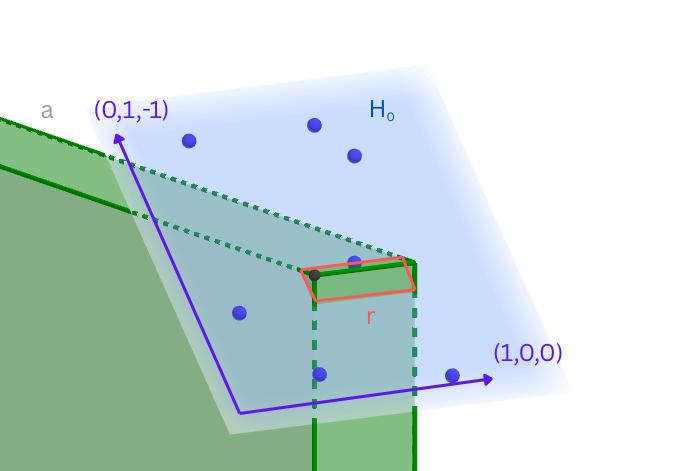
\includegraphics[width=0.7\textwidth]{sikvag2.png}
    \caption{Cutting out an axis-parallel rectangle of $H_0$}
    \label{ferde}
\end{figure}

Our goal is to show that $m_{\{p^iq^j:i,j \in \mathbb{N}\},\{0\}}(k) \geq m_{\mathcal{T}_{fin}}(k)$. 

We have already shown in the proof of Theorem \ref{vegtelen_sorozat}. (2) that 
$m_{\{p^iq^j:i,j \in \mathbb{N}\},\{0\}}^{\infty}(k) \geq m_{\mathcal{T}_3}(k)$. To every $T_A \in \mathcal{T}_3$, we have assigned a hypergraph $A \in \mathcal{A}_{D,\{0\}}^{\infty}$, $D = \{p^iq^j:i,j \in \mathbb{N}\}$ by an injection $\gamma_A: V(T_A) \to \mathbb{N}$ such that for every hyperedge (octant) $E\subseteq V(T_A)$ the vertex set (set of some natural numbers) $\gamma_A[E]$ was a hyperedge (arithmetic progression with proper difference $d_E$) in $A$. Observe that every set $E_{x_1,x_2,y_0,z_0} = \{(x,y,z): x_1 \leq x \leq x_2, \text{ } y \leq y_0, \text { } z \leq z_0\}$ is the subset of an octant $O_{x_1,y_0,z_0} = \{(x,y,z): x_1 \leq x, \text{ } y \leq y_0, \text { } z \leq z_0\}$. 

Therefore, for every $T_{A'} \in \mathcal{T}_{fin}$ we have a $T_A \in \mathcal{T}_3$ such that $V(T_A) = V(T_{A'})$, and every hyperedge in $T_{A'}$ is the subset of a hyperedge of $T_A$. Use the same $\gamma_A$ injection to obtain a hypergraph $A' \in \mathcal{A}_{D,\{0\}}$. The image of every octant $O_{x_1,y_0,z_0} \cap V(T_A)$ is (the subset of) an arithmetic progresson with some $a_0$ and difference $d=p^iq^j$. Notice that $a_0$ is divisible by $d$. Take a hyperedge $E = E_{x_1,x_2,y_0,z_0} \cap V(T_{A'})$ of $T_{A'}$ with an arbitrary $x_2 \in \mathbb{R}$. The image $\gamma_A[E]$ is the prefix of the arithmetic progression above, with last element $a_n$. If $a_n = K \cdot d$ then $\gamma_A[E] = \{k \cdot d: k \in \mathbb{N}^+, k \leq K\} \cap V(A')$, which can be a hyperedge in $A'$.
Therefore, $m_{\{p^iq^j:i,j \in \mathbb{N}\},\{0\}}(k) \geq m_{\mathcal{T}_{fin}}(k) = \infty$.
\end{proof}

\begin{thebibliography}{99}
\bibitem{teglalap}
X.~Chen, J.~Pach, M.~Szegedy, and G.~Tardos.
\newblock Delaunay graphs of point sets in the plane with respect to
  axis-parallel rectangles.
\newblock {\em Random Structures \& Algorithms}, 34(1):11--23, 2009.
\end{thebibliography}
\end{document}
